\usetikzlibrary{patterns}

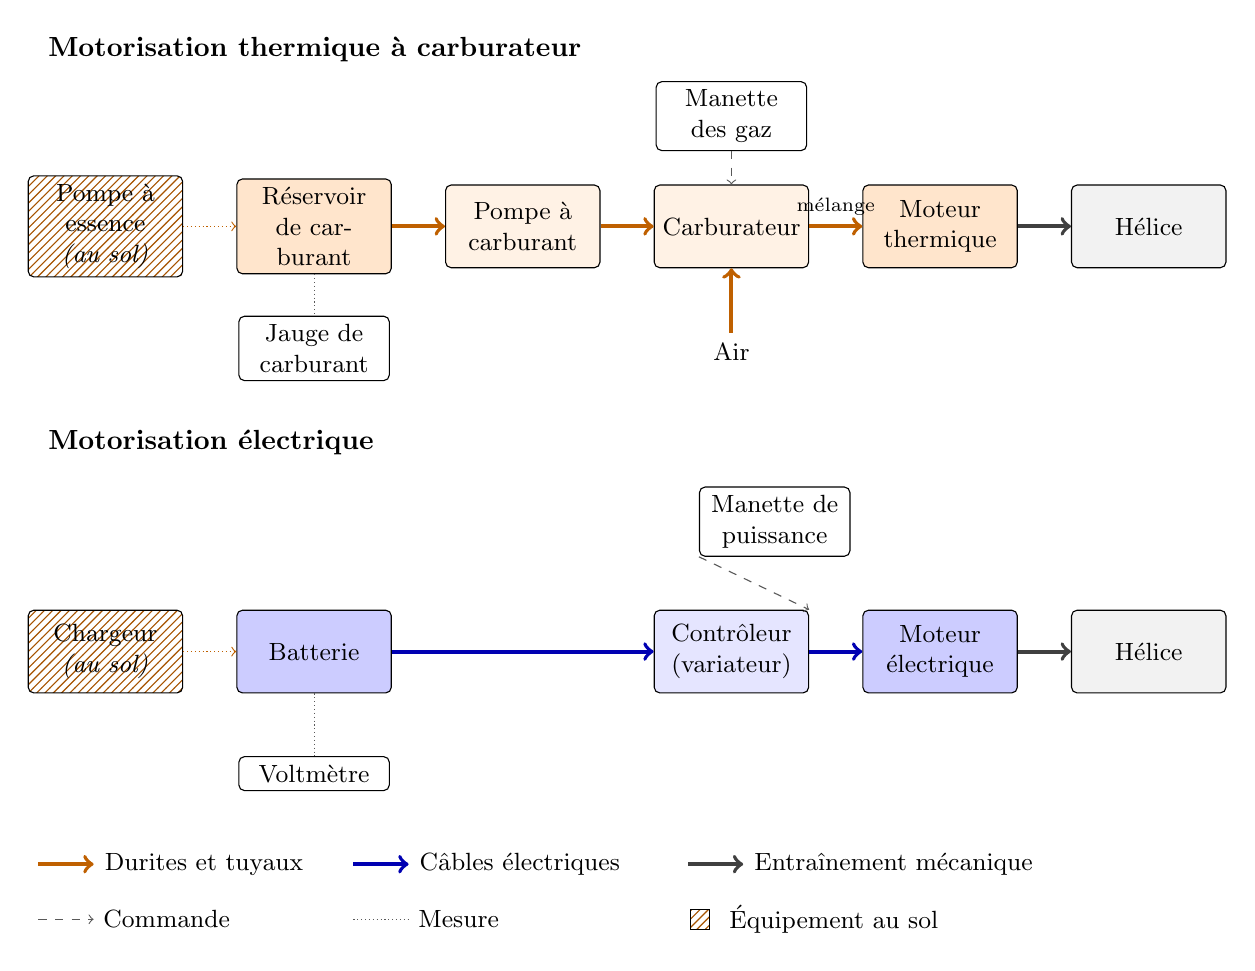
\begin{tikzpicture}[
    font=\small,
    element/.style={draw, rounded corners=2pt, minimum height=1.05cm,
        text width=1.75cm, align=center, inner sep=3pt},
    carburant/.style={draw=orange!75!black, line width=1.4pt, ->},
    electrique/.style={draw=blue!70!black, line width=1.4pt, ->},
    mecanique/.style={draw=black!75, line width=1.4pt, ->},
    commande/.style={draw=black!65, dashed, ->},
    mesure/.style={draw=black!65, densely dotted},
    transfertSol/.style={draw=orange!75!black, densely dotted, ->},
    equipementSol/.style={element, fill=orange!8,
        pattern=north east lines, pattern color=orange!65!black},
    instrument/.style={draw, rounded corners=2pt, fill=white,
        text width=1.7cm, align=center, inner sep=3pt}
]
    \node[anchor=west, font=\bfseries] at (-0.85,2.25)
        {Motorisation thermique à carburateur};

    \node[equipementSol] (station) at (0,0) {Pompe à essence\\\textit{(au sol)}};
    \node[element, fill=orange!20] (reservoir) at (2.65,0) {Réservoir\\de carburant};
    \node[element, fill=orange!10] (pompe) at (5.3,0) {Pompe à\\carburant};
    \node[element, fill=orange!10] (carburateur) at (7.95,0) {Carburateur};
    \node[element, fill=orange!20] (thermique) at (10.6,0) {Moteur\\thermique};
    \node[element, fill=gray!10] (heliceT) at (13.25,0) {Hélice};

    \draw[transfertSol] (station.east) -- (reservoir.west);
    \draw[carburant] (reservoir.east) -- (pompe.west);
    \draw[carburant] (pompe.east) -- (carburateur.west);
    \draw[carburant] (carburateur.east) -- node[above, font=\scriptsize] {mélange} (thermique.west);
    \draw[mecanique] (thermique.east) -- (heliceT.west);

    \node[instrument] (jauge) at (2.65,-1.55) {Jauge de\\carburant};
    \draw[mesure] (reservoir.south) -- (jauge.north);
    \node[instrument] (gaz) at (7.95,1.4) {Manette\\des gaz};
    \draw[commande] (gaz.south) -- (carburateur.north);
    \draw[carburant] (7.95,-1.35) node[below, text=black] {Air} -- (carburateur.south);

    \node[anchor=west, font=\bfseries] at (-0.85,-2.75)
        {Motorisation électrique};

    \node[equipementSol] (chargeur) at (0,-5.4) {Chargeur\\\textit{(au sol)}};
    \node[element, fill=blue!20] (batterie) at (2.65,-5.4) {Batterie};
    \node[element, fill=blue!10] (controleur) at (7.95,-5.4) {Contrôleur\\(variateur)};
    \node[element, fill=blue!20] (moteurE) at (10.6,-5.4) {Moteur\\électrique};
    \node[element, fill=gray!10] (heliceE) at (13.25,-5.4) {Hélice};

    \draw[transfertSol] (chargeur.east) -- (batterie.west);
    \draw[electrique] (batterie.east) -- (controleur.west);
    \draw[electrique] (controleur.east) -- (moteurE.west);
    \draw[mecanique] (moteurE.east) -- (heliceE.west);

    \node[instrument] (voltmetre) at (2.65,-6.95) {Voltmètre};
    \draw[mesure] (batterie.south) -- (voltmetre.north);
    \node[instrument] (puissance) at (8.5,-3.75) {Manette de\\puissance};
    \draw[commande] (puissance.south west) -- (controleur.north east);

    \draw[carburant] (-0.85,-8.1) -- ++(0.7,0)
        node[right, text=black] {Durites et tuyaux};
    \draw[electrique] (3.15,-8.1) -- ++(0.7,0)
        node[right, text=black] {Câbles électriques};
    \draw[mecanique] (7.4,-8.1) -- ++(0.7,0)
        node[right, text=black] {Entraînement mécanique};
    \draw[commande] (-0.85,-8.8) -- ++(0.7,0)
        node[right, text=black] {Commande};
    \draw[mesure] (3.15,-8.8) -- ++(0.7,0)
        node[right, text=black] {Mesure};
    \node[draw, fill=orange!8, pattern=north east lines,
        pattern color=orange!65!black, minimum size=0.25cm] at (7.55,-8.8) {};
    \node[anchor=west] at (7.8,-8.8) {Équipement au sol};
\end{tikzpicture}
